\section{SQL-Parser}

\subsection{über den SQL-Parser: ZQL}

	Auf der Webseite vom \cite{zql1} Projekt ist der Open-Source-Parser ZQL zu finden, welcher in der Lage ist SQL zu parsen und in Datenstrukturen zu überführen. Der Parser selbst ist mit \cite{javacc1} geschrieben, einem  Java-Parsergenerator (zu vergleichen mit dem populärem Unix yacc Generator).

ZQL bietet Unterstützung für \verb|SELECT-|, \verb|INSERT-|, \verb|DELETE-|, \verb|COMMIT-|, \verb|ROLLBACK-|, \verb|UPDATE-|, \verb|SET|- und \verb|TRANSACTION-|Ausdrücke. Wichtig für diese Arbeit sind dabei insbesondere \verb|SELECT-| und \verb|UPDATE-|Ausdrücke, sowie -- die leider nicht enthaltenen -- \verb|CREATE TABLE-|Ausdrücke.

\subsection{Funktionsweise des Parsers}
\label{subsec:funktionparser}

ZQL kennt zwei grundlegende Interfaces \verb|ZExp| und \verb|ZStatement|. Wichtig für die weiterführende Erklärung ist, dass genau drei Klassen das Interface \verb|ZExp| implementieren. Diese werden im Folgenden auch vorgestellt. Es handelt sich um \verb|ZExpression, ZConstant, ZQuery|.

Das Interface \verb|ZStatement| bildet eine abstrakte Oberklasse für alle möglichen Arten von SQL-Statements. Folgende Klassen implementieren dieses Interface in ZQL:

\begin{itemize}
\item \verb|ZDelete| - repräsentiert ein \verb|DELETE| Statement
\item \verb|ZInsert| - repräsentiert ein \verb|INSERT| Statement
\item \verb|ZUpdate| - repräsentiert ein \verb|UPDATE| Statement
\item \verb|ZLockTable| - repräsentiert ein \verb|SQL LOCK TABLE| Statement
\item \verb|ZQuery| - repräsentiert ein \verb|SELECT| Statement
\end{itemize}

Das Interface \verb|ZExp| bildet eine abstrakte Oberklasse für drei verschiedene Arten von Ausdrücken:

\begin{itemize}
\item \verb|ZConstant| - Konstanten vom Typ \verb|NULL, NUMBER, STRING, COLUMNNAME| oder \verb|UNKNOWN|. Spaltennamen gehören hier also zu Konstanten im Sinne eines Parserbaumes. Im ZQL-Parserbaum sind Elemente entweder eine SQL-Anfrage (Query), ein Ausdruck, bestehend aus Operator und Operanden, oder eine Konstante. Spaltennamen fallen in die Kategorie Konstanten, da sie keine Ausdrücke oder SQL-Anfragen sind. 
\item \verb|ZExpression| - Ein SQL-Ausdruck bestehend aus einem Operator und einen oder mehreren Operanden
\item \verb|ZQuery| - Eine \verb|SELECT| Anfrage ist auch ein Ausdruck
\end{itemize}

Wir klären in diesem Abschnitt nun genauer, wie der Parser SQL-Anfragen in interne Datenstrukturen überführt.
Dazu müssen die Datentypen des Parserpaketes zunächst erläutert werden. Anschließend stellen wir eine Beispielanfrage und ihre Überführung in die Datenstrukturen des Parsers vor. Daraus leiten wir auch die Schwächen bzw. Grenzen des Parsers ab. Wir stellen im Folgenden dar, was für relevante Attribute und Methoden die jeweiligen Klassen besitzen. Da viele Klassen durch Vererbung entstehen, werden wir der Übersicht halber auch abgeleitete relevante Attribute und Funktionen mit einbeziehen. 

Wir verwenden im Folgenden eine Art Pseudocode. Elemente in einem Array oder Vector werden einfach als Menge \verb|{elem1, elem2, elem3}| dargestellt. Objekte werden vereinfacht dargestellt als Ansammlung von Attributen. Dies ist legitim, da die Methoden fast ausschließlich nur getter und setter sind. Ein Objekt o mit dem Attribut ``name'' und den Wert ``Otto'' schreiben wir daher als: 
\verb|o = { [name=Otto] }|

Die Klasse \textbf{ZFromItem} bezeichnet genau eine Tupelvariable samt Relation. Gespeichert wird in dieser Klasse daher der \textit{Name der Relation} und eine mögliche Tupelvariable als \textit{Alias}.

Der Aufbau der Klasse \textbf{ZSelectItem} ist komplexer. Sie ist verantwortlich Spaltennamen, Konstanten, Tupelvariablen, Ausdrücke und Aggregationsfunktionen zu speichern. Bevor wir den Aufbau dieser Klasse an einem Beispiel verdeutlichen, gehen wir jetzt alle Attribute dieser Klasse im Detail ein.

%\begin{figure}[h]
\begin{tabular}{lp{.8\textwidth}}
\verb|wildcard| & Haben wir nur das Wildcard \verb|*| wird hier der boolsche Wert \verb|true| gespeichert, ansonsten ist dieser Wert \verb|false|.\\
\verb|aggregate| & Handelt es sich beim aktuellen Gegenstand um eine Aggregationsfunktion, so wird der Name dieser hier gespeichert.\\
\verb|alias| & Hier wird eine alternative Spaltenüberschrift als \verb|STRING| gespeichert.\\
\verb|columnname| & Hier wird der Spaltenname gespeichert. Ist eine Konstante angegeben, so wird diese hier ebenfalls gespeichert. Stringkonstanten werden dabei mit eingeschlossenen, doppelten Anführungszeichen gespeichert, damit sie von Spaltennamen unterschieden werden können. Numerische Konstanten werden als String gespeichert. Handelt es sich um einen zusammengesetzten Term, so wird dieser hier gespeichert. In jedem Fall werden Tupelvariablen nicht im Attribut \verb|columnname| gespeichert.\\
\verb|table| & In diesem Attribut wird die Tupelvariable abgespeichert. Haben wir in \verb|columnname| einen zusammengesetzten Term gespeichert, so werden die Tupelvariablen dieses Terms hier ebenso abgespeichert, indem die Spaltennamen aus dem Term entfernt werden. Deutlich wird dieses Vorgehen im folgenden Beispiel.\\
\verb|expression| & In diesem Attribut wird immer ein Term gespeichert. Dabei ist es nicht wichtig, ob dieser einfach oder zusammengesetzt ist. Er wird so gespeichert wie er vom Nutzer aufgeschrieben wurde, das bedeutet insbesondere, dass die Tupelvariablen nicht extrahiert worden sind.\\
\end{tabular}
%\caption{Aufbau der Klasse \textbf{ZSelectItem}}
%\label{fig:zselitem}
%\end{figure}

Folgendes Beispiel soll die Struktur von \verb|ZSelectItem| erläutern. Wir betrachten dazu den folgenden \verb|SELECT|-Ausdruck: \begin{verbatim}SELECT e.sal AS "Spalte1", "Konstante" AS "Spalte2, 
e.sal + x.empno AS "Spalte3", avg(e.sal) AS "Spalte"4\end{verbatim} Um das Beispiel übersichtlich zu gestalten, geben wir nur Attribute an, die nicht leer sind oder vom Standardwert abweichen.

\begin{figure}[h]
\begin{verbatim}
{ [alias=Spalte1], [columnname=sal], [table=e], [expression=e.sal] }
{ [alias=Spalte2], [columnname="Konstante"], [expression="Konstante"] }
{ [alias=Spalte3], [columnname=empno], [table=e + x], 
  [expression=e.sal + x.empno] }
{ [aggregate = "avg"], [alias=Spalte4], [columnname=sal], [table=e], 
  [expression=avg(e.sal)] }
\end{verbatim}
\caption{Geparste Objekte vom Typ \textbf{ZSelectItem}}
\end{figure}

Der \verb|WHERE|-Teil wird dargestellt mit Hilfe der Klasse \textbf{ZExpression}. Diese Klasse implementiert das Interface \verb|ZExp|. Ein Objekt der Klasse \verb|ZExpression| besteht immer aus einem Operator und mehreren Operanden. Ein Operator ist ein gültiger String. Ein Ausdruck speichert seine Operanden als \textit{Vector} von Objekten, die das Interface \verb|ZExp| implementieren. Demnach kann ein Operand vom Typ \verb|ZExpression, ZConstant| oder \verb|ZQuery| sein.
Wichtig ist auch zu bemerken, dass ZQL nicht nur zwei Operanden pro Ausdruck kennt. 

Ein üblicher Syntaxbaum ist binär, wobei die Wurzel den Operator mit der höchsten Priorität darstellt. Alle Teilbäume sind als Ausdrücke zu verstehen, jeweils mit Operator als Wurzelknoten und Operanden als Kindknoten. Dabei kann ein Operand auch ein weiterer Ausdruck sein. Generell wird dabei das Prinzip der Assoziativität benutzt um \mbox{z. B.} für gleichrangige Operatoren eine Auswertungsreihenfolge festzulegen.

So würde der \verb|WHERE|-Teil von folgender SQL-Anfrage:
\begin{verbatim}
SELECT * FROM emp e WHERE e.sal > 1000 AND e.sal < 2000 AND e.id > 1234
\end{verbatim}

zu folgendem, geklammerten Ausdruck werden:
\begin{verbatim}
(((e.sal > 1000) AND (e.sal < 2000)) AND (e.id > 1234))
\end{verbatim}

\begin{figure}[h]
\label{baum1}
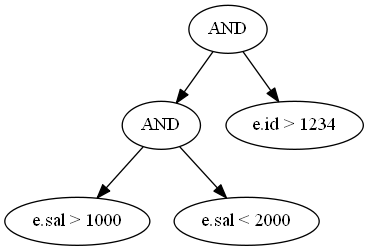
\includegraphics[scale=0.7]{Bilder/where_syntax.png}
\caption{WHERE-Bedingung in üblichen Syntaxbäumen}
\end{figure}

Der ZQL-Parser funktioniert so allerdings nicht. Wird keine spezielle Klammerung benutzt, so werden gleichrangige Operatoren nicht assoziativ geklammert, sondern befinden sich auf einer Ebene des Baumes. Somit handelt es sich nicht um einen binären Baum. 

Wir erhalten also aus obigen \verb|WHERE|-Ausdruck:
\begin{verbatim}
((e.sal > 1000) AND (e.sal < 2000) AND (e.id > 1234))
\end{verbatim}

\begin{figure}
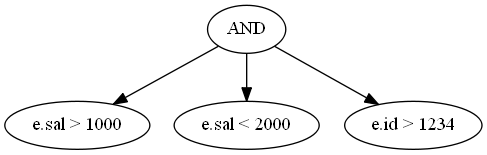
\includegraphics[scale=0.7]{Bilder/with_zql.png}
\caption{WHERE-Bedingung geparst mit ZQL}
\end{figure}
%ende baumerklaerung

So erklärt sich auch die Verwendung eines \textit{Vector} zur Speicherung der Operanden.

Die Klasse \textbf{ZConstant} dient zur Darstellung von SQL-Konstanten. Sie speichert den Wert der Konstante sowie den Typ. Als Typen kommen in Frage: \verb|NULL, NUMBER, STRING, UNKNOWN, COLUMNNAME|. Spaltennamen zählen hier auch zu Konstanten, da ein Spaltenname kein Operator mit Operanden ist, was einer \verb|ZExpression| entsprechen würde.

Ein Objekt der Klasse \textbf{ZGroupBy} speichert im Wesentlichen zwei Informationen. Die \verb|GROUP BY| Ausdrücke werden gespeichert in einem \textit{Vector} von Klassen, die das \verb|ZExp| Interface implementiert haben. Der optionale \verb|HAVING BY| Ausdruck wird als Objekt einer der Klassen gespeichert, welche \verb|ZExp| implementieren. Typischerweise wird das ein Objekt der Klasse \verb|ZExpression| sein.

Die Klasse \textbf{ZOrderBy} speichert einzelne Sortierkriterien. Gebündelt werden diese dann über einen \textit{Vector}. Ein Objekt der Klasse \verb|ZOrderBy| enthält einen Ausdruck vom Typ \verb|ZExp| sowie die Information ob nach dem Suchkriterium aufsteigend oder absteigend sortiert werden soll.

Letztendlich vereinigt die Klasse \textbf{ZQuery} die eben vorgestellten Klassen. Die Funktion \verb|getSelect()| liefert einen \textit{Vector} von \verb|ZSelectItem| zurück. Ähnlich dazu liefert die Methode \verb|getFrom()| einen \textit{Vector} von \verb|ZFromItem| zurück. Hier erkennt man schon eine Beschränkung des Parsers. Da der \verb|FROM|-Teil nur als Ansammlung von \verb|FROM|-Items abstrahiert wird, werden Joins unter \verb|FROM| nicht vom Parser erfasst. Die Methode \verb|getWhere()| liefert ein Objekt zurück, was das Interface \verb|ZExp| implementiert haben muss. Typischerweise ist dies ein Objekt der Klasse \verb|ZExpression|. Analog dazu liefert die Methode \verb|getGroupBy()| ein Objekt der Klasse \verb|ZGroupBy| zurück. Die Methode \verb|getOrderBy| liefert einen \textit{Vector} von \verb|ZOrderBy|-Objekten zurück.
Schlussendlich existiert noch eine Methode \verb|isDistinct()|, die klärt ob ein \verb|DISTINCT| verwendet wurde.

Dies sind die am häufigsten gebrauchten Klassen des ZQL-Parser. Wir wollen nun die Arbeitsweise des Parsers anhand eines Beispieles verdeutlichen. Da die \verb|SELECT|-Anfragen die wohl am häufigsten gebrauchte Form der Anfragen ist, wird sich die Erklärung der Funktionsweise des Parsers beispielhaft auf diese Art der Anfragen beziehen. Wie die anderen Statements geparst werden ist dann analog schnell zu verstehen.


Eine gewöhnliches Select-Statement wird wie folgt vom Parser zerlegt:
\begin{verbatim}
SELECT e.name, sal, dname 
FROM emp e, dept d 
WHERE e.sal > 1000 AND e.did = d.id 
ORDER BY e.sal DESC\end{verbatim}

Die ganze Anfrage wird in einem Objekt vom Typ \verb|ZQuery| eingebettet. Wir gehen nun nacheinander die Bestandteile dieses Objektes durch. 

Der \textbf{SELECT}-Teil wird durch einen \textit{Vector} dargestellt. Alle Items sind vom Typ \textit{ZSelectItem}. \verb|SelectVector = { sel1, sel2, sel3 }|.

\verb|sel1 = { [Table=e], [Column=name], [Expression=e.name], [Wildcard=false] }|

\verb|sel2 = { [Column=sal], [Expression=sal], [Wildcard=false] }|

\verb|sel3 = { [Column=dname], [Expression=dname], [Wildcard=false] }|

Auch im \verb|FROM|-Teil finden wir einen \textit{Vector}, der nun aus Objekten vom Typ \verb|ZFromItem| besteht. \verb|FromVector = { fromItem1, fromItem2 }|.

\verb|fromItem1 = { [Table=emp], [Alias=e] }|\\
\verb|fromItem2 = { [Table=dept], [Alias=d] }|

Kommen wir nun zum komplexeren Teil, dem \verb|WHERE|-Ausdruck. Da diese Struktur baumartig ist, lässt sich dies zunächst besser in einem Bild ausdrücken.

\begin{figure}[h]
\centering
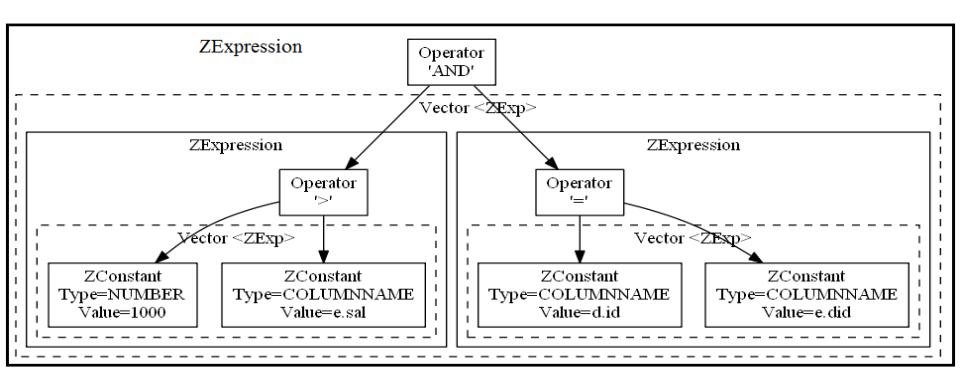
\includegraphics[scale=0.51]{Bilder/where_teil.png}
\caption{Geparster Baum der WHERE Bedingung des Beispiels}
\label{fig:parseTree}
\end{figure}

In Abbildung \ref{fig:parseTree} sieht man nun den geparsten Baum der \verb|WHERE|-Bedingung. Die gestrichelten K"asten sollen andeuten, dass es sich um den \textit{Vector} von Klassen handelt, die \verb|ZExp| implementieren, während durchgezogene Kasten konkrete Objekte sein sollen.

Der \verb|ORDER BY|-Teil wird wiederum als \textit{Vector} von \textit{ZOrderBy}-Objekten gspeichert.\\
\verb|OrderByVector = { orderBy1 }|.

\verb|orderBy1 = { [asc = false], [expression = e.sal] }|

\subsection{Grenzen des Parsers}
\label{subsec:grenzenparser}

Der Parser kann keine \verb|CREATE TABLE|-Statements parsen. Somit ist es im Rahmen dieser Arbeit notwendig, den Parser zu erweitern, damit Tabellen in eigene Datenstrukturen geparst werden können. Für die Arbeit ist es zunächst nur notwendig Name, Datentyp, Fremdschlüsselbeziehungen und NULL-Informationen der Spalten in eine interne Datenstruktur zu überführen. Dabei wird beim Typ nur zwischen Zahlen und Sonstigem (Text) unterschieden. Wir speichern außerdem, wie viele Nachkommastellen ein Attribut haben kann. Unser Programm soll in der Lage sein, einfache arithmetische Operationen durchzuführen. Dazu ist das Wissen um Datentypen der Variablen von Nöten.

Der ZQL-Parser versteht das \verb|FROM|-Statement als Liste von Relationen mit optionalen Tupelvariablen. Dadurch leiten sich mehrere Einschränkungen ab. ZQL ist dadurch nicht in der Lage \verb|JOINS| über die Schlüsselworte \\\verb#  ON [LEFT OUTER|RIGHT OUTER|INNER] JOIN# \\zu erkennen. Der Parser erkennt nur innere \verb|JOINS|, die im \verb|WHERE|-Teil formuliert worden. Der ZQL-Parser unterstützt daher auch keine Unterabfragen unter \verb|FROM|. Eine Möglichkeit diesem Problem zu begegnen ist es, solche Unterabfragen vor dem Parsen zu Entfernen und danach unverändert wieder einzufügen. Es wäre allerdings wünschenswerter wenn der ZQL-Parser erweitert würde, so dass auch ein \verb|ZQuery| als \verb|ZFromItem| benutzt werden kann.

Trotz dieser Einschränkungen sind alle Konzepte, die in dieser Arbeit vorgestellt werden einfach auf jedweden SQL-Parser übertragbar.

%TODO: CREATE TABLE

\section{JavaServer Pages}

JavaServer Pages (JSP), ist eine auf JHTML basierende Web-Programmiersprache zur dynamischen Erzeugung von HTML- oder XML-Dokumenten auf einem Webserver. Im Jahre 1999 wurden die JSP von Sun Microsystems veröffentlicht. Man kann sich die JSP als High-Level Abstraktion eines Java Servlets vorstellen. JSP werden zur Laufzeit in Servlets umgewandelt. Jedes dieser JSP-Servlets wird gecached und wiederverwendet, bis die Original-JSP verändert wurde. Ein skizzenhaftes Schema, finden wir in Abbildung \ref{fig:jsp}

\begin{figure}[h]
\begin{subfigure}[b]{.4\textwidth}
 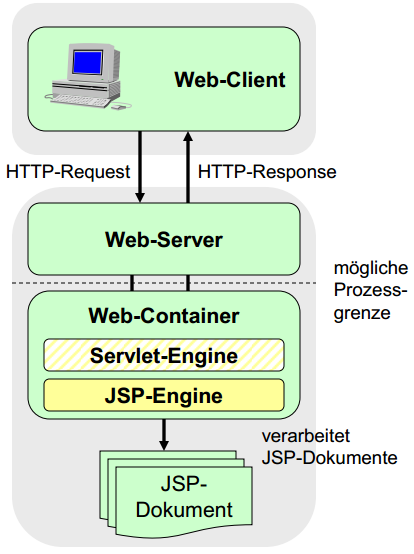
\includegraphics[scale=0.3]{Bilder/jsp.png}
 \caption{JSP-Konzep}
 \label{fig:jsp}
\end{subfigure}
\begin{subfigure}[b]{.5\textwidth}
\begin{tabular}{|l|l|}
\hline
\textbf{Objekt} & \textbf{Typ} \\\hline
request	& javax.servlet.http.HttpServletRequest \\\hline
response & javax.servlet.http.HttpServletResponse \\\hline
session & javax.servlet.http.HttpSession \\\hline
pageContext	& javax.servlet.jsp.PageContext \\\hline
application	& javax.servlet.ServletContext \\\hline
config& javax.servlet.ServletConfig \\ \hline
out	& javax.servlet.jsp.JspWriter \\\hline
exception & java.lang.Throwable \\\hline
\end{tabular}
\caption{Implizte Objekte in JSP}
\label{fig:implicitObj}
\end{subfigure}
\caption{}
\end{figure}


Man könnte die JSP als Erweiterung der Servlets ansehen, da die JSP alle Funktionen dieser übernehmen. Zusätzlich können auch eigene Tag-Libraries erstellt werden. JSP funktioniert ähnlich wie ASP oder PHP. Sowohl Java-Servlets, als auch die JSP, haben die Aufgabe die Ausführung von Javacode dem Nutzer  per HTML verfügbar zu machen. Im Gegensatz zu den Java-Servlets, die komplett aus Javacode bestehen, bestehen JSP-Dateien aus HTML mit kurzen Einschüben von Javacode. Während man also bei den Servlets HTML-Ausgaben nur innerhalb einer Funktion bewerkstelligen kann, ist es möglich bei den JSP direkt HTML auszuschreiben.

\subsection{Funktionsweise}

Wie bereits erwähnt, handelt es sich bei einer JSP-Seite um ein HTML-Dokument. Daher gibt es hier keine expliziten Funktionen oder Klassen, die die Ausgabe eines Javaprogrammes steuern. Stattdessen stehen dem Programmierer unter JSP mehrere implizite Objekte zur Verfügung, um deren Konstruktion er sich nicht kümmern muss. Eine Übersicht der impliziten Objekte finden wir in Abbildung \ref{fig:implicitObj}. Da eine JSP-Datei im eigentlichem Sinne eine (J)HTML-Seite ist, muss der Javacode abgegrenzt werden. Wir schreiben sämtlichen Javacode daher innerhalb von \verb|<% %>|. Diese Funktionieren ähnlich wie \verb|<?php ?>| in PHP.

Wir gehen nun kurz auf wesentliche implizite Objekte ein. Das Objekt \textbf{request} beinhaltet alle Funktionen und Daten, die wir benötigen um die HTTP-Anfrage zu verarbeiten. Wir haben \mbox{z. B.} Zugriff auf: Cookies, HTTP-Header, übertragene POST- oder GET-Variablen (hier Parameter genannt).

Das \textbf{response}-Objekt ist das genaue Gegenstück zum request-Objekt. Es enthält alle Informationen für die HTTP-Response und wird vor allem genutzt, um den Content-Type festzulegen und Response-Header oder Cookies zu setzen. 

Das \textbf{session}-Objekt regelt alle wichtigen Funktionen für die aktuelle Session. Wir können hier die Session-ID abfragen, sowie Objekte zur Session hinzufügen und entfernen.

Als letztes, möchten wir das \textbf{out}-Objekt erwähnen. Es repräsentiert einen BufferedWriter, genauer JSPWriter. Das Objekt kennt im Wesentlichen die Funktionen \verb|print| und \verb|println|. In PHP entspricht dies einem \verb|echo| oder \verb|print| Befehl. Der so gedruckte Text, wird zur Laufzeit in die entstehende HTML-Datei geschrieben. 

Das folgende Beispiel soll die Verwendung der impliziten Objekte verdeutlichen, ist aber, aus Platzgründen, stark vereinfacht.
\lstset{language=Java}
\begin{lstlisting}
<%@page import="java.util.Date"%>
<%@page language="java" contentType="text/html" 
		pageEncoding="UTF-8" %>
<html xmlns="http://www.w3.org/1999/xhtml">
<head><title>Datum: <% out.print(new Date()); %></title></head>
<body>Zu dieser Seite sind 
<% out.print(request.getCookies().length); %> 
Cookies gespeichert.
</body></html>
\end{lstlisting}

\section{Auflistung der Software}

Um die Programmierung nachzuvollziehen wird im Folgenden die verwendete Software aufgelistet. Wir vermerken dabei Name, Version, Kurzbeschreibung sowie die Webpräsenz der Software.

\begin{tabular}{p{10cm}r}
\textbf{Software}: ZQL-Parser & \textbf{Version}: 2011-08-26\\
\multicolumn{2}{p{1\textwidth}}{\textbf{Beschreibung}: Ein Open-Source-Parser, der mit JavaCC, einem Java-Parser-Generator, realisiert wurde. Wir haben bereits einige Schwächen bemerkt, er ist aber leicht erweiterbar, da er quelloffen ist und unter der GNU GPLv3 steht.}\\
\multicolumn{2}{l}{\textbf{URL}: \url{http://zql.sourceforge.net/}}
\end{tabular}\\

\begin{tabular}{p{10cm}r}
\textbf{Software}: Apache Tomcat & \textbf{Version}:6.0\\
\multicolumn{2}{p{1\textwidth}}{\textbf{Beschreibung}: Tomcat ist ein Webserver, der in einem Web-Container die Servlet- und die JSP-Engine bereithält. Mit ihm ist es möglich, JSP-Seiten zu betreiben.}\\
\multicolumn{2}{l}{\textbf{URL}: \url{http://tomcat.apache.org/}}
\end{tabular}\\

\begin{tabular}{p{10cm}r}
\textbf{Software}: Oracle JDK  & \textbf{Version}:1.6.0\\
\multicolumn{2}{p{1\textwidth}}{\textbf{Beschreibung}: Das Java-JDK ist notwendig um Programme zu übersetzen und auszuführen. Wir verwenden Version 1.6.0, da im universitärem Umfeld, in dessen Rahmen unser Programm entsteht, häufig noch diese Version verwendet wird. Unser Programm ist jedoch auch kompatibel zu JDK 1.7.0.}\\
\multicolumn{2}{l}{\textbf{URL}: \url{http://www.oracle.com/technetwork/java/javase/downloads/index.html}}
\end{tabular}\\

\begin{tabular}{p{10cm}r}
\textbf{Software}: JDBC-Connector für MySQL  & \textbf{Version}:5.1.25\\
\multicolumn{2}{p{1\textwidth}}{\textbf{Beschreibung}: Java Database Connectivity (JDBC) ist eine Datenbankschnittstelle der Java-Plattform, die eine einheitliche Schnittstelle zu Datenbanken verschiedener Hersteller bietet und speziell auf relationale Datenbanken ausgerichtet ist. JDBC ist in seiner Funktion als universelle Datenbankschnittstelle vergleichbar mit z. B. ODBC unter Windows oder DBI unter Perl. Zu den Aufgaben von JDBC gehört es, Datenbankverbindungen aufzubauen und zu verwalten, SQL-Anfragen an die Datenbank weiterzuleiten und die Ergebnisse in eine für Java nutzbare Form umzuwandeln und dem Programm zur Verfügung zu stellen. Für jede spezifische Datenbank sind eigene Treiber erforderlich, die die JDBC-Spezifikation implementieren. Diese Treiber werden meist vom Hersteller des Datenbank-Systems geliefert.}\\
\multicolumn{2}{l}{\textbf{URL}: \url{http://dev.mysql.com/downloads/connector/j/}}
\end{tabular}\\

\begin{tabular}{p{10cm}r}
\textbf{Software}: JDBC-Connector für PostgreSQL  & \textbf{Version}:9.2-1003\\
\multicolumn{2}{p{1\textwidth}}{\textbf{Beschreibung}: siehe JDBC-Connector für MySQL}\\
\multicolumn{2}{l}{\textbf{URL}: \url{http://jdbc.postgresql.org/download.html}}
\end{tabular}\\

\begin{tabular}{p{10cm}r}
\textbf{Software}: JDBC-Connector für Oracle Database & \textbf{Version}:-\\
\multicolumn{2}{p{1\textwidth}}{\textbf{Beschreibung}: siehe JDBC-Connector für MySQL}\\
\multicolumn{2}{l}{\textbf{URL}: \url{http://www.oracle.com/technetwork/database/features/jdbc/index-091264.html}}
\end{tabular}\\